\chapter{Nodes and Packet Forwarding}
\label{chap:nodes}

This chapter describes one aspect of creating a topology in \ns,
\ie, creating the nodes.
In 
\href{the next chapter}{Chapter}{chap:links},
we will describe second aspect of creating the topology,
\ie, connecting the nodes to form links.
% This chapter does not describe the detailed internal organization of
% a node (although some schematics are given), nor the interaction
% between a node and its routing modules; please refer to
% Chapter~\ref{chap:rtarch} for detailed discussion.

Recall that each simulation requires a single instance of the
\clsref{Simulator}{../ns-2/tcl/lib/ns-lib.tcl} to control and operate
that simulation. 
The class provides instance procedures to create and manage the topology,
and internally stores references to each element of the topology.
We begin 
\href{by describing the procedures in the class Simulator}{%
        Section}{sec:node:simulator}.
We then
\href{describe the instance procedures in the class Node}{%
        Section}{sec:node:node}
to access and operate on individual nodes.
We conclude
\href{with detailed descriptions of the Classifier}{%
        Section}{sec:node:classifiers}
from which the more complex node objects are formed.

The procedures and functions described in this chapter can be found in
\nsf{tcl/lib/ns-lib.tcl}, \nsf{tcl/lib/ns-node.tcl}, \\
\nsf{tcl/lib/ns-rtmodule.tcl}, \nsf{rtmodule.\{cc,h\}}, 
\nsf{classifier.\{cc, h\}}, \nsf{classifier-addr.cc},
\nsf{classifier-mcast.cc}, \nsf{classifier-mpath.cc}, 
and, \nsf{replicator.cc}.

\section{Node Basics}
\label{sec:node:simulator}

The basic primitive for creating a node is
\begin{program}
    set ns [new Simulator]
    $ns \fcnref{\textbf{node}}{../ns-2/ns-lib.tcl}{Simulator::node}
\end{program} %$
The instance procedure \code{node} constructs
a node out of more simple
\href{classifier objects}{Section}{sec:node:classifiers}.
The Node itself is a standalone class in OTcl.
However, most of the components of the node are themselves TclObjects.
The typical structure of a (unicast) 
node is as shown in Figure~\ref{fig:node:unicast}.  This simple structure
consists of two TclObjects:  an address classifer (\code{classifer_}) and
a port classifier (\code{dmux_}).  The function of these classifiers
is to distribute incoming packets to the correct agent or outgoing link.
\begin{figure}[tb]
  \centerline{\includegraphics{node}}
  \caption{Structure of a Unicast Node.  Notice that entry\_ is simply a 
   label variable instead of a real object, e.g., the classifier\_.}
  \label{fig:node:unicast}
\end{figure}

All nodes contain at least the following components:
\begin{itemize}
\item an address or \code{id_}, monotonically increasing by 1 (from 
initial value 0) across the simulation namespace as nodes are created,
\item a list of neighbors (\code{neighbor_}),
\item a list of agents (\code{agent_}),
\item a node type identifier (\code{nodetype_}), and
\item a routing module (described in Section~\ref{sec:node:rtarch} below)
\end{itemize}

% PLEASE NOTE THAT ADDRESS EXPAND COMMAND IS NOW DEPRECATED SINCE NODE AND PORT
% ADDRESS SPACES WERE EXPANDED TO 32 BITS.
% Before \ns\ release 2.1b6, the address of an agent in a node is 16
% bits wide: the higher 8 bits define the node \code{id_},
% the lower 8 bits identify the individual agent at the node.
% This limits the number of nodes in a simulation to 256 nodes.
% If the user needs to create a topology larger than 256 nodes,
% then they should first expand the address space before creating any
% nodes, as
% \begin{program}
%         $ns set-address-format expanded
% \end{program} %$
% This expands the address space to 30 bits, the higher 22 of which are 
% used to assign node numbers.
% 
% \framebox{
%   \begin{minipage}{\textwidth}
%     {\bf Note}: Starting from release 2.1b6, the above is no longer
%     necessary; \ns\ uses 32-bit integers for both address and port.
%     Therefore, the above restriction of 256 nodes is no longer applicable.
%   \end{minipage}
% }

By default, nodes in \ns\ are constructed for unicast simulations.
In order to enable multicast simulation, the simulation should be created 
with an option ``-multicast on'', e.g.:
\begin{program}
        set ns [new Simulator -multicast on]
\end{program}
% {\bf NOTE}: the old way of enabling multicast,
%         e.g., \code{Simulator set EnableMcast_ 1},
%         is no longer needed.
The internal structure of a typical multicast node is shown in
Figure~\ref{fig:node:multicast}.
\begin{figure}
  \centerline{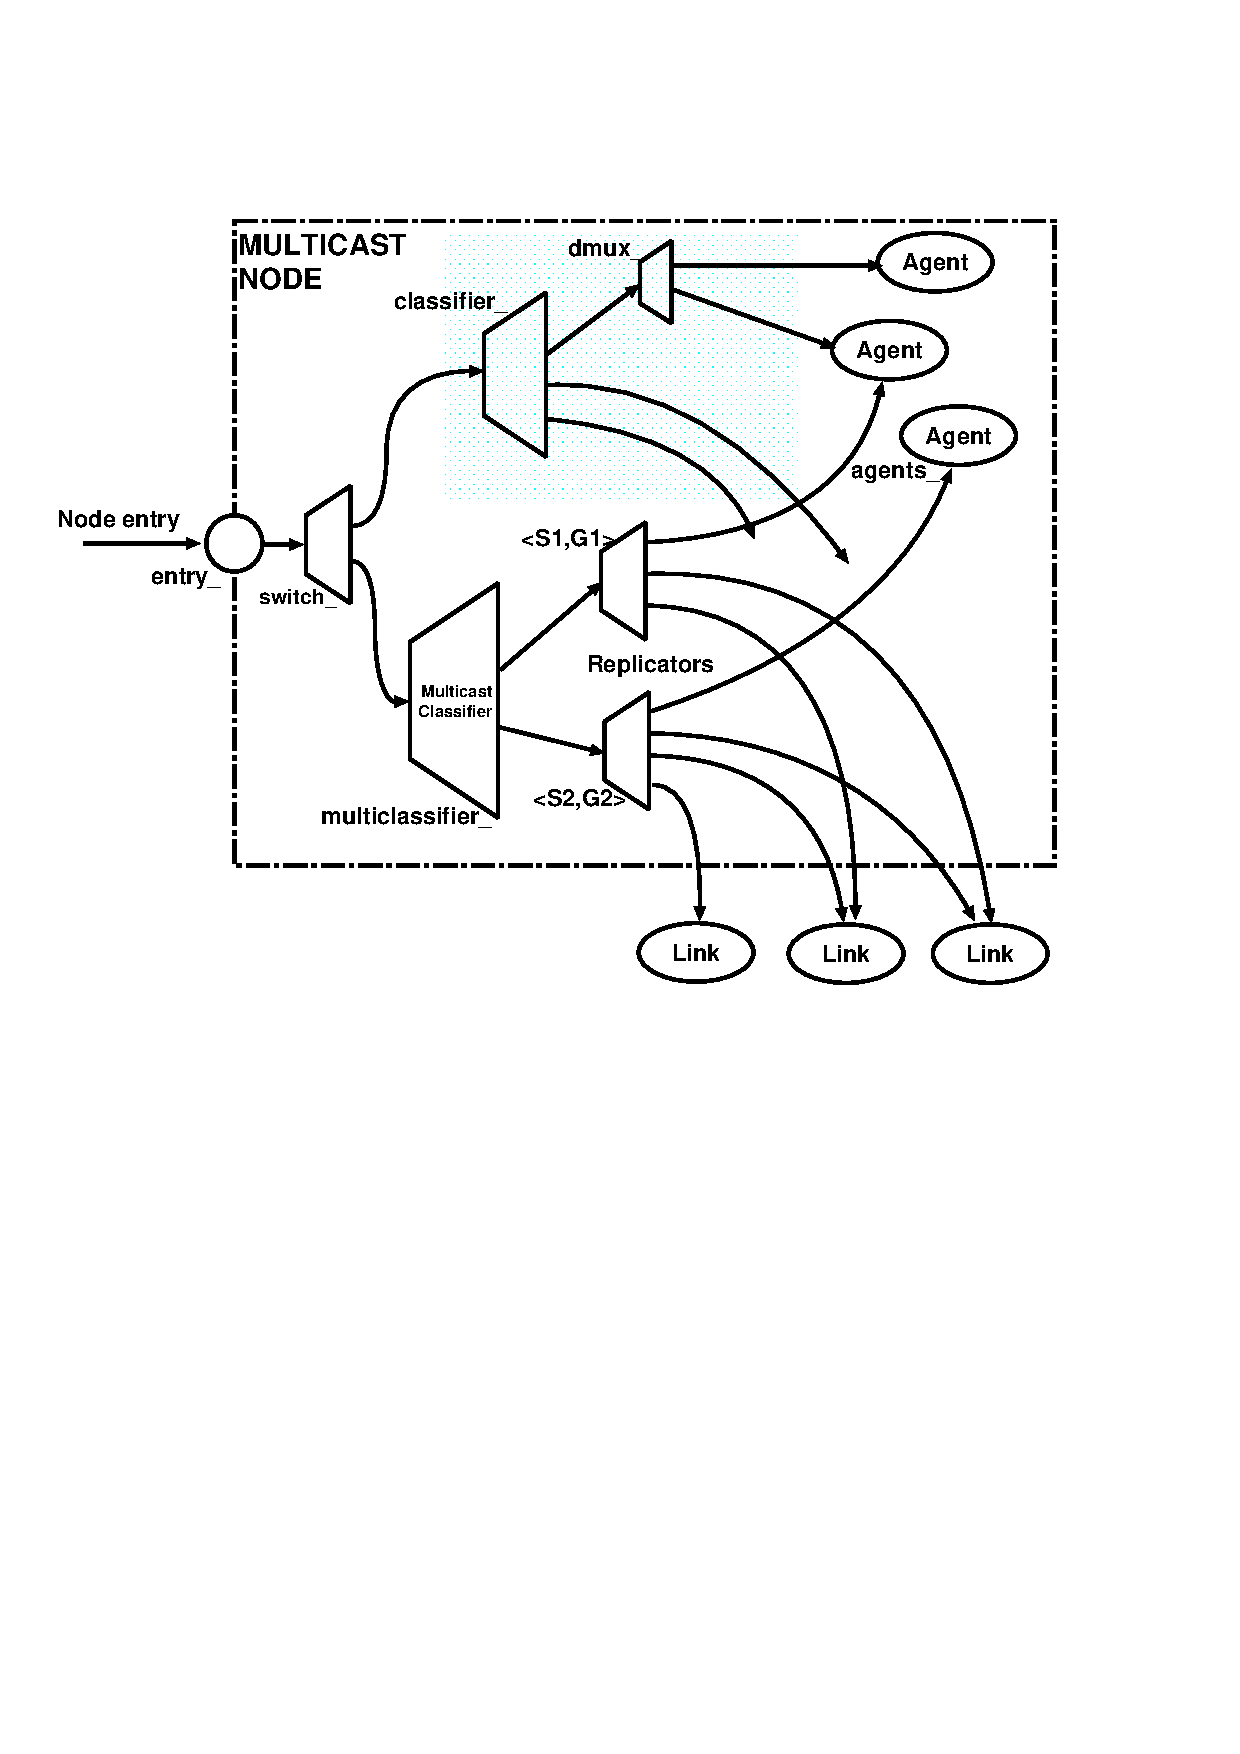
\includegraphics{mcastNode}}
  \caption{Internal Structure of a Multicast Node.}
  \label{fig:node:multicast}
\end{figure}

When a simulation uses multicast routing,
the highest bit of the address indicates whether the particular
address is a multicast address or an unicast address.
If the bit is 0, the address represents a unicast address,
else the address represents a multicast address.
% This implies that, by default, 
% a multicast simulation is restricted to 128 nodes.

\section{Node Methods: Configuring the Node}
\label{sec:node:node}

Procedures to configure an individual node can be classified into:
\begin{list}{---}{\itemsep0pt}
\item Control functions
\item Address and Port number management, unicast routing functions
\item Agent management
\item Adding neighbors
\end{list}
We describe each of the functions in the following paragraphs.

\paragraph{Control functions}
\begin{enumerate}
\item \code{$node entry} %$
returns the entry point for a node.
This is the first element which will handle packets arriving at that node.

The Node instance variable, \code{entry_}, stores the reference this element.
For unicast nodes, this is the address classifier that looks at the higher
bits of the destination address.
The instance variable, \code{classifier_} contains the reference to this
classifier.
However, for multicast nodes, the entry point is the
\code{switch_} which looks at the first bit to decide whether
it should forward the packet to the unicast classifier, or the multicast
classifier as appropriate.

\item \code{$node reset} %$
will reset all agents at the node.
\end{enumerate}


\paragraph{Address and Port number management}
The procedure \code{$node id} %$
returns the node number of the node.
This number is automatically incremented and assigned to each node at
creation by the class Simulator method, \code{$ns node}.%$
The class Simulator also stores an instance variable array\footnote{%
  \ie, an instance variable of a class that is also an array variable},
  \code{Node_}, indexed by the node id, and contains a reference to the
  node with that id.

The procedure \code{$node agent \tup{port}} %$
returns the handle of the
agent at the specified port.
If no agent at the specified port number is available, the procedure returns
the null string.

The procedure \code{alloc-port} returns the next available port number.
It uses an instance variable, \code{np_},
to track the next unallocated port number.

The procedures, \code{add-route} and \code{add-routes},
are used by \href{unicast routing}{Chapter}{chap:unicast}
to add routes to populate the \code{classifier_}
The usage syntax is
\code{$node add-route \tup{destination id} \tup{TclObject}}. %$
\code{TclObject} is the entry of \code{dmux_}, the port demultiplexer
at the node, if the destination id is the same as this node's id,
it is often the head of a link to send packets for that destination to,
but could also be the the entry for other classifiers or types of classifiers.

\code{$node add-routes \tup{destination id} \tup{TclObjects}} %$
is used to add multiple routes to the same destination that must be used
simultaneously in round robin manner to spread the bandwidth used to reach
that destination across all links equally.
It is used only if the instance variable \code{multiPath_} is set to 1,
and detailed dynamic routing strategies are in effect,
and requires the use of a multiPath classifier.
We describe the implementation of the multiPath classifier
\href{later in this chapter}{Section}{sec:node:classifiers};
however, \href{we defer the discussion of multipath
routing}{Chapter}{chap:unicast} to the chapter on unicast routing.

The dual of \proc[]{add-routes} is \proc[]{delete-routes}.
It takes the id, a list of \code{TclObjects}, and a reference to
the simulator's \code{nullagent}.
It removes the TclObjects in the list from the installed routes in the
multipath classifier.
If the route entry in the classifier does not point to a multipath
classifier,
the routine simply clears the entry from \code{classifier_}, and
installs the \code{nullagent} in its place.

Detailed dynamic routing also uses two additional methods:
the instance procedure \proc[]{init-routing} sets the instance variable
\code{multiPath_} to be equal to the class variable of the same name.
It also adds a reference to the route controller object at that node
in the instance variable, \code{rtObject_}.
The procedure \proc[]{rtObject?} returns the handle for the route object 
at the node.

Finally, the procedure \proc[]{intf-changed} is invoked by
the network dynamics code if a link incident on the node
changes state.  Additional details on how this procedure
is used are discussed later
\href{in the chapter on network dynamics}{Chapter}{chap:net-dynamics}.

\paragraph{Agent management}
Given an \tup{agent}, the procedure \proc[]{attach} will
add the agent to its list of \code{agents_},
assign a port number the agent and set its source address,
set the target of the agent to be its (\ie, the node's) \proc[]{entry},
and add a pointer to the port demultiplexer at the node (\code{dmux_})
to the agent at the corresponding slot in the \code{dmux_} classifier.

Conversely, \proc[]{detach}will remove the agent from \code{agents_},
and point the agent's target, and the entry in the node \code{dmux_}
to \code{nullagent}.

\paragraph{Tracking Neighbors}
Each node keeps a list of its adjacent neighbors in its instance variable,
\code{neighbor_}.  The procedure \proc[]{add-neighbor} adds a neighbor to the list.  The procedure \proc[]{neighbors} returns this list.

\section{Node Configuration Interface}
\label{sec:node:nodeconfig}

\framebox{
  \begin{minipage}{\textwidth}
    {\bf NOTE}: This API, especially its internal implementation which
    is messy at this point, is still a moving target. It may undergo
    significant changes in the near future. However, we will do our
    best to maintain the same interface as described in this chapter.
    In addition, this API currently does not cover all existing nodes
    in the old format, namely, nodes built using inheritance, and
    parts of mobile IP. It is principally oriented towards wireless
    and satellite simulation.
    [Sep 15, 2000; updated June 2001].
  \end{minipage}
}

\proc[]{Simulator::node-config} accommodates flexible and modular
construction of different node definitions within the same base Node
class.
For instance, to create a mobile node capable
of wireless communication, one no longer needs a specialized node
creation command, e.g., \proc[]{dsdv-create-mobile-node}; instead, one
changes default configuration parameters, such as  
\begin{program}
$ns node-config -adhocRouting dsdv 
\end{program}
before actually 
creating the node with the command: \code{$ns node}.
Together with routing modules, this allows
one to combine ``arbitrary'' routing functionalities within a single
node without resorting to multiple inheritance and other fancy object
gimmicks. 
We will describe this in more detail in Section~\ref{sec:node:rtarch}.
The functions and procedures relevant to the new node APIs may be
found in \nsf{tcl/lib/ns-node.tcl}.

The node configuration interface consists of two parts. 
The first part deals with node configuration, while the second part
actually creates nodes of the specified type. 
We have already seen the latter in Section~\ref{sec:node:simulator},
in this section we will describe the configuration part. 

Node configuration essentially consists of defining the different node
characteristics before creating them. They may consist of the type of
addressing structure used in the simulation, defining the network
components for mobilenodes, turning on or off the trace options at
Agent/Router/MAC levels, selecting the type of adhoc routing protocol for
wireless nodes or defining their energy model.

As an example, node-configuration for a wireless, mobile node that 
runs AODV as its
adhoc routing protocol in a hierarchical topology would be as shown below.
We decide to turn tracing on at the agent and router level only. Also we 
assume a topology has been instantiated with "set topo [new Topography]". 
The node-config command would look like the following:

\begin{program}
  \$ns_ node-config -addressType hierarchical \bs 
                   -adhocRouting AODV \bs
                   -llType LL \bs
                   -macType Mac/802_11 \bs 
                   -ifqType Queue/DropTail/PriQueue \bs
                   -ifqLen 50 \bs
                   -antType Antenna/OmniAntenna \bs 
                   -propType Propagation/TwoRayGround \bs
                   -phyType Phy/WirelessPhy \bs
                   -topologyInstance \$topo \bs
                   -channel Channel/WirelessChannel \bs 
                   -agentTrace ON \bs 
                   -routerTrace ON \bs
                   -macTrace OFF \bs
                   -movementTrace OFF 
\end{program}

The default values for all the above options are NULL except 
\code{-addressingType}
whose default value is flat. The option \code{-reset} can be used to reset all
node-config parameters to their default value.

Note that the config command can be broken down into separate lines like
\begin{program}
        \$ns_ node-config -addressingType hier
        \$ns_ node-config -macTrace ON
\end{program}
The options that need to be changed may only be called. For example after
configuring for AODV mobilenodes as shown above (and after creating AODV
mobilenodes), we may configure for AODV base-station nodes in the
following way: 
\begin{program}
        \$ns_ node-config -wiredRouting ON
\end{program}
While all other features for base-station nodes and mobilenodes are same,
the base-station nodes are capable of wired routing, while mobilenodes are
not. In this way we can change node-configuration only when it is required.

All node instances created after a given node-configuration command will
have the same property unless a part or all of the node-config command is
executed with different parameter values. And all parameter values remain
unchanged unless they are expicitly changed. So after creation of the AODV
base-station and mobilenodes, if we want to create simple nodes, we will
use the following node-configuration command:
\begin{program}
        \$ns_ node-config -reset
\end{program}
This will set all parameter values to their default setting which
basically defines configuration of a simple node.

Currently, this type of node configuration is oriented towards wireless
and satellite nodes.  Table 5.1
%% ~\ref{table:nodeconfig} 
lists the available options
for these kinds of nodes.  The example scripts 
\nsf{tcl/ex/simple-wireless.tcl} and \nsf{tcl/ex/sat-mixed.tcl} provide
usage examples.

\begin{table}[ht]
\label{table:nodeconfig}
\begin{center} 
{\footnotesize
\begin{tabular}{|l|l|l|}\hline
{\bf option} & {\bf available values} & {\bf default}\\\hline\hline 
\multicolumn{3}{|c|}{\bf general} \\\hline
{\bf addressType} & flat, hierarchical & flat\\\hline
{\bf MPLS} & ON, OFF & OFF\\\hline
\multicolumn{3}{|c|}{\bf both satellite- and wireless-oriented} \\\hline
{\bf wiredRouting} & ON, OFF & OFF\\\hline
{\bf llType} & LL, LL/Sat & "" \\\hline
{\bf macType} & Mac/802\_11, Mac/Csma/Ca, Mac/Sat, & \\ 
& Mac/Sat/UnslottedAloha, Mac/Tdma & "" \\\hline
{\bf ifqType} & Queue/DropTail, Queue/DropTail/PriQueue & "" \\\hline
{\bf phyType} & Phy/WirelessPhy, Phy/Sat& "" \\\hline
\multicolumn{3}{|c|}{\bf wireless-oriented} \\\hline
{\bf adhocRouting} & DIFFUSION/RATE, DIFFUSION/PROB, DSDV, & \\
& DSR, FLOODING, OMNIMCAST, AODV, TORA & ""\\\hline
{\bf propType} & Propagation/TwoRayGround, Propagation/Shadowing & ""\\\hline
{\bf propInstance} & Propagation/TwoRayGround, Propagation/Shadowing & ""\\\hline
{\bf antType} & Antenna/OmniAntenna & ""\\\hline
{\bf channel} & Channel/WirelessChannel, Channel/Sat & ""\\\hline
{\bf topoInstance} & <topology file> & ""\\\hline
{\bf mobileIP} & ON, OFF& OFF \\\hline
{\bf energyModel} & EnergyModel & "" \\\hline
{\bf initialEnergy} & <value in Joules> & "" \\\hline
{\bf rxPower} & <value in W> & "" \\\hline
{\bf txPower} & <value in W> & "" \\\hline
{\bf idlePower} & <value in W> & "" \\\hline
{\bf agentTrace} & ON, OFF & OFF \\\hline
{\bf routerTrace} & ON, OFF & OFF \\\hline
{\bf macTrace} & ON, OFF & OFF \\\hline
{\bf movementTrace} & ON, OFF & OFF \\\hline
{\bf errProc} & UniformErrorProc & "" \\\hline
{\bf FECProc} &? & ? \\\hline
{\bf toraDebug} & ON, OFF & OFF \\\hline
\multicolumn{3}{|c|}{\bf satellite-oriented} \\\hline
{\bf satNodeType} & polar, geo, terminal, geo-repeater & "" \\\hline
{\bf downlinkBW} & <bandwidth value, e.g. "2Mb"> & ""\\\hline
\end{tabular}
}
\end{center}
\caption{Available options for node configuration (see tcl/lib/ns-lib.tcl).
}
\end{table}
\normalsize

\section{The Classifier}
\label{sec:node:classifiers}

The function of a node when it receives a packet is to examine
the packet's fields, usually its destination address, and
on occasion, its source address.
It should then map the values to an outgoing interface object
that is the next downstream recipient of this packet.

In \ns, this task is performed by a simple \emph{classifier} object.
Multiple classifier objects,
each looking at a specific portion of the packet
forward the packet through the node.
A node in \ns\ uses many different types of classifiers for different purposes.
This section describes some of the more common, or simpler,
classifier objects in \ns.

We begin with a description of the base class in this section.
The next subsections describe
\href{the address classifier}{Section}{sec:node:addr-classifier},
\href{the multicast classifier}{Section}{sec:node:mcast-classifier},
\href{the multipath classifier}{Section}{sec:node:mpath-classifier}, 
\href{the hash classifier}{Section}{sec:node:hash-classifier}, and
finally, \href{the replicator}{Section}{sec:node:replicator}.

A classifier provides a way to match a packet against some
logical criteria and retrieve a reference to another simulation
object based on the match results.
Each classifier contains a table of simulation objects indexed
by {\em slot number}.
The job of a classifier is to determine the slot number associated
with a received packet and forward that packet to the
object referenced by that particular slot.
The C++ \clsref{Classifier}{../ns-2/classifier.h}
(defined in \nsf{classifier.h})
provides a base class from which other classifiers are derived.
\begin{program}
        class Classifier : public NsObject \{
        public:
                ~Classifier();
                void recv(Packet*, Handler* h = 0);
         protected:
                Classifier();
                void install(int slot, NsObject*);
                void clear(int slot);
                virtual int command(int argc, const char*const* argv);
                virtual int classify(Packet *const) = 0;
                void alloc(int);
                NsObject** slot_;       \* table that maps slot number to a NsObject */
                int nslot_;
                int maxslot_;
        \};
\end{program}
The \fcn[]{classify} method is pure virtual, indicating the
class \code{Classifier} is to be used only as a base class.
The \fcn[]{alloc} method dynamically allocates enough space
in the table to hold the specified number of slots.
The \fcn[]{install} and \fcn[]{clear} methods
add or remove objects from the table.
The \fcn[]{recv} method and the OTcl interface are implemented
as follows in \nsf{classifier.cc}:
\begin{program}
        /*
         *{\cf objects only ever see "packet" events, which come either}
         *{\cf from an incoming link or a local agent (i.e., packet source).}
         */
        void Classifier::recv(Packet* p, Handler*)
        \{
                NsObject* node;
                int cl = classify(p);
                if (cl < 0 || cl >= nslot_ || (node = slot_[cl]) == 0) \{
                        Tcl::instance().evalf("%s no-slot %d", name(), cl);
                        Packet::free(p);
                        return;
                \}
                node->recv(p);
        \}

        int Classifier::command(int argc, const char*const* argv)
        \{
                Tcl& tcl = Tcl::instance();
                if (argc == 3) \{
                        /*
                         * $classifier clear $slot
                         */
                        if (strcmp(argv[1], "clear") == 0) \{
                                int slot = atoi(argv[2]);
                                clear(slot);
                                return (TCL_OK);
                        \}
                        /*
                         * $classifier installNext $node
                         */
                        if (strcmp(argv[1], "installNext") == 0) \{
                                int slot = maxslot_ + 1;
                                NsObject* node = (NsObject*)TclObject::lookup(argv[2]);
                                install(slot, node);
                                tcl.resultf("%u", slot);
                                return TCL_OK;
                        \}
                        if (strcmp(argv[1], "slot") == 0) \{
                                int slot = atoi(argv[2]);
                                if ((slot >= 0) || (slot < nslot_)) \{
                                        tcl.resultf("%s", slot_[slot]->name());
                                        return TCL_OK;
                                \}
                                tcl.resultf("Classifier: no object at slot %d", slot);
                                return (TCL_ERROR);
                        \}
                \} else if (argc == 4) \{
                        /*
                         * $classifier install $slot $node
                         */
                        if (strcmp(argv[1], "install") == 0) \{
                                int slot = atoi(argv[2]);
                                NsObject* node = (NsObject*)TclObject::lookup(argv[3]);
                                install(slot, node);
                                return (TCL_OK);
                        \}
                \}
                return (NsObject::command(argc, argv));
        \}
\end{program} %$
When a classifier \fcn[]{recv}'s a packet,
it hands it to the \fcn[]{classify} method.
This is defined differently in each type of classifier
derived from the base class.
The usual format is for the \fcn[]{classify} method to
determine and return a slot index into the table of slots.
If the index is valid, and points to a valid TclObject,
the classifier will hand the packet to that object using 
that object's \fcn[]{recv} method.
If the index is not valid, the classifier will invoke
the instance procedure \proc[]{no-slot} to attempt to 
populate the table correctly.
However, in the base class \proc[]{Classifier::no-slot} prints
and error message and terminates execution.

The \fcnref{\fcn[]{command} method}{../ns-2/classifier.cc}{Classifier::command}
provides the following instproc-likes to the interpreter:
\begin{itemize}\itemsep0pt
\item \proc[\tup{slot}]{clear} clears the entry in a particular slot.
\item \proc[\tup{object}]{installNext} installs the object
        in the next available slot, and returns the slot number.

        Note that this instproc-like is 
        \fcnref{overloaded by an instance procedure of the same name}{%
                ../ns-2/ns-lib.tcl}{Classifier::installNext}
        that stores a reference to the object stored.
        This then helps quick query of the objects
        installed in the classifier from OTcl.
\item \proc[\tup{index}]{slot} returns the object stored in the specified slot.
\item \proc[\tup{index}, \tup{object}]{install} installs the specified
        \tup{object} at the slot \tup{index}.

        Note that this instproc-like too is 
        \fcnref{overloaded by an instance procedure of the same name}{%
                ../ns-2/ns-lib.tcl}{Classifier::install}
        that stores a reference to the object stored.
        This is also to quickly query of the objects
        installed in the classifier from OTcl.
\end{itemize}

\subsection{Address Classifiers}
\label{sec:node:addr-classifier}

An address classifier is used in supporting unicast packet forwarding.
It applies a bitwise shift and mask operation to a packet's destination
address to produce a slot number.
The slot number is returned from the \fcn[]{classify} method.
The \clsref{AddressClassifier}{../ns-2/classifier-addr.cc}
(defined in \nsf{classifier-addr.cc}) ide defined as follows:
\begin{program}
        class AddressClassifier : public Classifier \{
        public:
                AddressClassifier() : mask_(~0), shift_(0) \{
                        bind("mask_", (int*)&mask_);
                        bind("shift_", &shift_);
                \}
        protected:
                int classify(Packet *const p) \{
                        IPHeader *h = IPHeader::access(p->bits());
                        return ((h->dst() >> shift_) & mask_);
                \}
                nsaddr_t mask_;
                int shift_;
        \};
\end{program}
The class imposes no direct semantic meaning
on a packet's destination address field.
Rather, it returns some number of bits from the packet's
\code{dst_} field as the slot number used
in the \fcnref{\fcn[]{Classifier::recv}}{../ns-2/classifier.cc}{Classifier::recv} method.
The \code{mask_} and \code{shift_} values are set through OTcl.

\subsection{Multicast Classifiers}
\label{sec:node:mcast-classifier}

The multicast classifier classifies packets
according to both source and destination (group) addresses.
It maintains a (chained hash) table mapping source/group pairs to slot numbers.
When a packet arrives containing a source/group unknown to the classifier,
it invokes an Otcl procedure \proc[]{Node::new-group}
to add an entry to its table.
This OTcl procedure may use the method \code{set-hash} to add
new (source, group, slot) 3-tuples to the classifier's table.
The multicast classifier is defined in \nsf{classifier-mcast.cc}
as follows:
\begin{program}
        static class MCastClassifierClass : public TclClass \{
        public:
                MCastClassifierClass() : TclClass("Classifier/Multicast") \{\}
                TclObject* create(int argc, const char*const* argv) \{
                        return (new MCastClassifier());
                \}
        \} class_mcast_classifier;

        class MCastClassifier : public Classifier \{
        public:
                MCastClassifier();
                ~MCastClassifier();
        protected:
                int command(int argc, const char*const* argv);
                int classify(Packet *const p);
                int findslot();
                void set_hash(nsaddr_t src, nsaddr_t dst, int slot);
                int hash(nsaddr_t src, nsaddr_t dst) const \{
                        u_int32_t s = src ^ dst;
                        s ^= s >> 16;
                        s ^= s >> 8;
                        return (s & 0xff);
                \}
                struct hashnode \{
                        int slot;
                        nsaddr_t src;
                        nsaddr_t dst;
                        hashnode* next;
                \};
                hashnode* ht_[256];
                const hashnode* lookup(nsaddr_t src, nsaddr_t dst) const;
        \};

        int MCastClassifier::classify(Packet *const pkt)
        \{
                IPHeader *h = IPHeader::access(pkt->bits());
                nsaddr_t src = h->src() >> 8; /*XXX*/
                nsaddr_t dst = h->dst();
                const hashnode* p = lookup(src, dst);
                if (p == 0) \{
                        /*
                         * Didn't find an entry.
                         * Call tcl exactly once to install one.
                         * If tcl doesn't come through then fail.
                         */
                        Tcl::instance().evalf("%s new-group %u %u", name(), src, dst);
                        p = lookup(src, dst);
                        if (p == 0)
                                return (-1);
                \}
                return (p->slot);
        \}
\end{program}
The \clsref{MCastClassifier}  implements a chained hash table
and applies a hash function on both the packet source and
destination addresses.
The hash function returns the slot number
to index the \code{slot_} table in the underlying object.
A hash miss implies packet delivery to a previously-unknown group;
OTcl is called to handle the situation.
The OTcl code is expected to insert an appropriate entry into the hash table.

\subsection{MultiPath Classifier}
\label{sec:node:mpath-classifier}

This object is devised to support equal cost multipath
forwarding, where the node has multiple equal cost routes
to the same destination, and would like to use all of them
simultaneously.
This object does not look at any field in the packet.
With every succeeding packet, 
it simply returns the next filled slot in round robin fashion.
The definitions for this classifier are in \nsf{classifier-mpath.cc},
and are shown below:
\begin{program}
class MultiPathForwarder : public Classifier \{
public:
        MultiPathForwarder() : ns_(0), Classifier() \{\} 
        virtual int classify(Packet* const) \{
                int cl;
                int fail = ns_;
                do \{
                        cl = ns_++;
                        ns_ %= (maxslot_ + 1);
                \} while (slot_[cl] == 0 && ns_ != fail);
                return cl;
        \}
private:
        int ns_;     \* next slot to be used.  Probably a misnomer? */
\};
\end{program}

\subsection{Hash Classifier}
\label{sec:node:hash-classifier}

This object is used to classify a packet as a member of a
particular {\em flow}.
As their name indicates,
hash classifiers use a hash table internally to assign
packets to flows.
These objects are used where flow-level information is
required (e.g. in flow-specific queuing disciplines and statistics
collection).
Several ``flow granularities'' are available.  In particular,
packets may be assigned to flows based on flow ID, destination address,
source/destination addresses, or the combination of source/destination
addresses plus flow ID.
The fields accessed by the hash classifier are limited to
the {\tt ip} header: {\tt src(), dst(), flowid()} (see {\tt ip.h}).

The hash classifier is created with an integer argument specifying
the initial size of its hash table.  The current hash table size may
be subsequently altered with the {\tt resize} method (see below).
When created, the instance variables \code{shift_} and \code{mask_}
are initialized with the simulator's current {\sf NodeShift} and
{\sf NodeMask} values, respectively.  These values are retrieved
from the {\tt AddrParams} object when the hash classifier is
instantiated.  The hash classifier will fail to operate properly if
the {\tt AddrParams} structure is not initialized.
The following constructors are used for the various hash classifiers:
\begin{program}
        Classifier/Hash/SrcDest
        Classifier/Hash/Dest
        Classifier/Hash/Fid
        Classifier/Hash/SrcDestFid
\end{program}

The hash classifier receives packets, classifies them according
to their flow criteria, and retrieves the classifier {\em slot}
indicating the next node that should receive the packet.
In several circumstances with hash classifiers, most packets should
be associated with a single slot, while only a few flows should
be directed elsewhere. 
The hash classifier includes a \code{default_} instance variable
indicating which slot is to be used for packets that do not match
any of the per-flow criteria.
The \code{default_} may be set optionally.

The methods for a hash classifier are as follows:
\begin{program}
        $hashcl set-hash buck src dst fid slot
        $hashcl lookup buck src dst fid
        $hashcl del-hash src dst fid
        $hashcl resize nbuck
\end{program}

The \fcn[]{set-hash} method inserts a new entry into the hash
table within the hash classifier.
The {\tt buck} argument specifies the hash table bucket number
to use for the insertion of this entry.
When the bucket number is not known, {\tt buck} may be specified
as {\tt auto}. 
The {\tt src, dst} and {\tt fid} arguments specify the IP source,
destination, and flow IDs to be matched for flow classification.
Fields not used by a particular classifier (e.g. specifying {\tt src}
for a flow-id classifier) is ignored.
The {\tt slot} argument indicates the index into the underlying
slot table in the base {\tt Classifier} object from which
the hash classifier is derived.
The {\tt lookup} function returns the name of the object
associated with the given {\tt buck/src/dst/fid} tuple.
The {\tt buck} argument may be {\tt auto}, as for {\tt set-hash}.
The {\tt del-hash} function removes the specified entry from
the hash table.
Currently, this is done by simply marking the entry as inactive,
so it is possible to populate the hash table with unused entries.
The {\tt resize} function resizes the hash table to include
the number of buckets specified by the argument {\tt nbuck}.

Provided no default is defined, a hash classifier will
perform a call into OTcl when it
receives a packet which matches no flow criteria.
The call takes the following form:
\begin{program}
        \$obj unknown-flow src dst flowid buck
\end{program} 
Thus, when a packet matching no flow criteria is received,
the method {\tt unknown-flow} of the instantiated hash classifier
object is invoked with the source, destination, and flow id
fields from the packet.
In addition, the {\tt buck} field indicates the hash bucket
which should contain this flow if it were inserted using
{\tt set-hash}.  This arrangement avoids another hash
lookup when performing insertions into the classifier when the
bucket is already known.

\subsection{Replicator}
\label{sec:node:replicator}

The replicator is different from the other classifiers
we have described earlier,
in that it does not use the classify function.
Rather, it simply uses the classifier as a table of $n$ slots;
it overloads the \fcn[]{recv} method to produce $n$ copies
of a packet, that are delivered to all $n$ objects referenced in the table.

To support multicast packet forwarding, a classifier receiving a
multicast packet from source $S$
destined for group $G$ computes a hash function $h(S,G)$ giving
a ``slot number'' in the classifier's object table.
%Thus, the maximum size of the table is $O(|S|\times|G|)$.
In multicast delivery, the packet must be copied once for
each link leading to nodes subscribed to $G$ minus one.
Production of additional copies of the packet is performed
by a \code{Replicator} class, defined in \code{replicator.cc}:
\begin{program}
        /*
         * {\cf A replicator is not really a packet classifier but}
         * {\cf we simply find convenience in leveraging its slot table.}
         * {\cf (this object used to implement fan-out on a multicast}
         * {\cf router as well as broadcast LANs)}
         */
        class Replicator : public Classifier \{
        public:
                Replicator();
                void recv(Packet*, Handler* h = 0);
                virtual int classify(Packet* const) \{\};
        protected:
                int ignore_;
        \};

        void Replicator::recv(Packet* p, Handler*)
        \{
                IPHeader *iph = IPHeader::access(p->bits());
                if (maxslot_ < 0) \{
                        if (!ignore_)
                                Tcl::instance().evalf("%s drop %u %u", name(), 
                                        iph->src(), iph->dst());
                        Packet::free(p);
                        return;
                \}
                for (int i = 0; i < maxslot_; ++i) \{
                        NsObject* o = slot_[i];
                        if (o != 0)
                                o->recv(p->copy());
                \}
                /* {\cf we know that maxslot is non-null} */
                slot_[maxslot_]->recv(p);
        \}
\end{program}
As we can see from the code,
this class  does not really classify packets.
Rather, it replicates a packet, one for each entry in its table,
and delivers the copies to each of the nodes listed in the table.
The last entry in the table gets the ``original'' packet.
Since the \fcn[]{classify} method is pure virtual in the base class,
the replicator defines an empty \fcn[]{classify} method.

\section{Routing Module and Classifier Organization}
\label{sec:node:rtarch}

As we have seen, a \ns\ node is essentially a collection of
classifiers.
The simplest node (unicast) contains only one address classifier and
one port classifier, as shown in Figure~\ref{fig:node:unicast}.
When one extends the functionality of the node, more classifiers are added
into the base node, for instance, the multicast node shown in
Figure~\ref{fig:node:multicast}.
As more function blocks is added, and each of these blocks requires
its own classifier(s), it becomes important for the node to
provide a {\em uniform} interface to organize these classifiers and to
bridge these classifiers to the route computation blocks.

The classical method to handle this case is through class
inheritance.
For instance, if one wants a node that supports hierarchical routing,
one simply derive a Node/Hier from the base node and override the
classifier setup methods to insert hierarchical classifiers.
This method works well when the new function blocks are independent
and cannot be ``arbitrarily'' mixed. 
For instance, both hierarchical routing and ad hoc routing use their
own set of classifiers. 
Inheritance would require that we have Node/Hier that supports
the former, and Node/Mobile for the latter.
This becomes slightly problematic when one wants an ad hoc routing
node that supports hierarchical routing.
In this simple case one may use multiple inheritance to solve the
problem, but this quickly becomes infeasible as the number of such
function blocks increases. 

The only method to solve this problem is object composition. 
The base node needs to define a set of interfaces for classifier
access and organization. 
These interfaces should
\begin{itemize}
\item allow individual routing modules that implement
  their own classifiers to insert their classifiers into the node;
\item allow route computation blocks to populate routes to classifiers
  in all routing modules that need this information, 
\item provide a single point of management for existing routing modules. 
\end{itemize}
In addition, we should also define a uniform interface for routing
modules to connect to the node interfaces, so as to provide a
systematic approach to extending node functionality. 
In this section we will describe the design of routing modules as well
as that of the corresponding node interfaces.

\subsection{Routing Module}

In general, every routing implementation in \ns\ consists of three
function blocks: 
\begin{itemize}
\item {\em Routing agent} exchanges routing packet with neighbors, 
\item {\em Route logic} uses the information gathered by routing
  agents (or the global topology database in the case of static
  routing) to perform the actual route computation, 
\item {\em Classifiers} sit inside a Node. They use the computed
  routing table to perform packet forwarding.
\end{itemize}
Notice that when implementing a new routing protocol, one does not
necessarily implement all of these three blocks.
For instance, when one implements a link state routing protocol, one
simply implement a routing agent that exchanges information in the
link state manner, and a route logic that does Dijkstra on the
resulting topology database. 
It can then use the same classifiers as other unicast routing
protocols.

\begin{figure}[tb]
  \begin{center}
    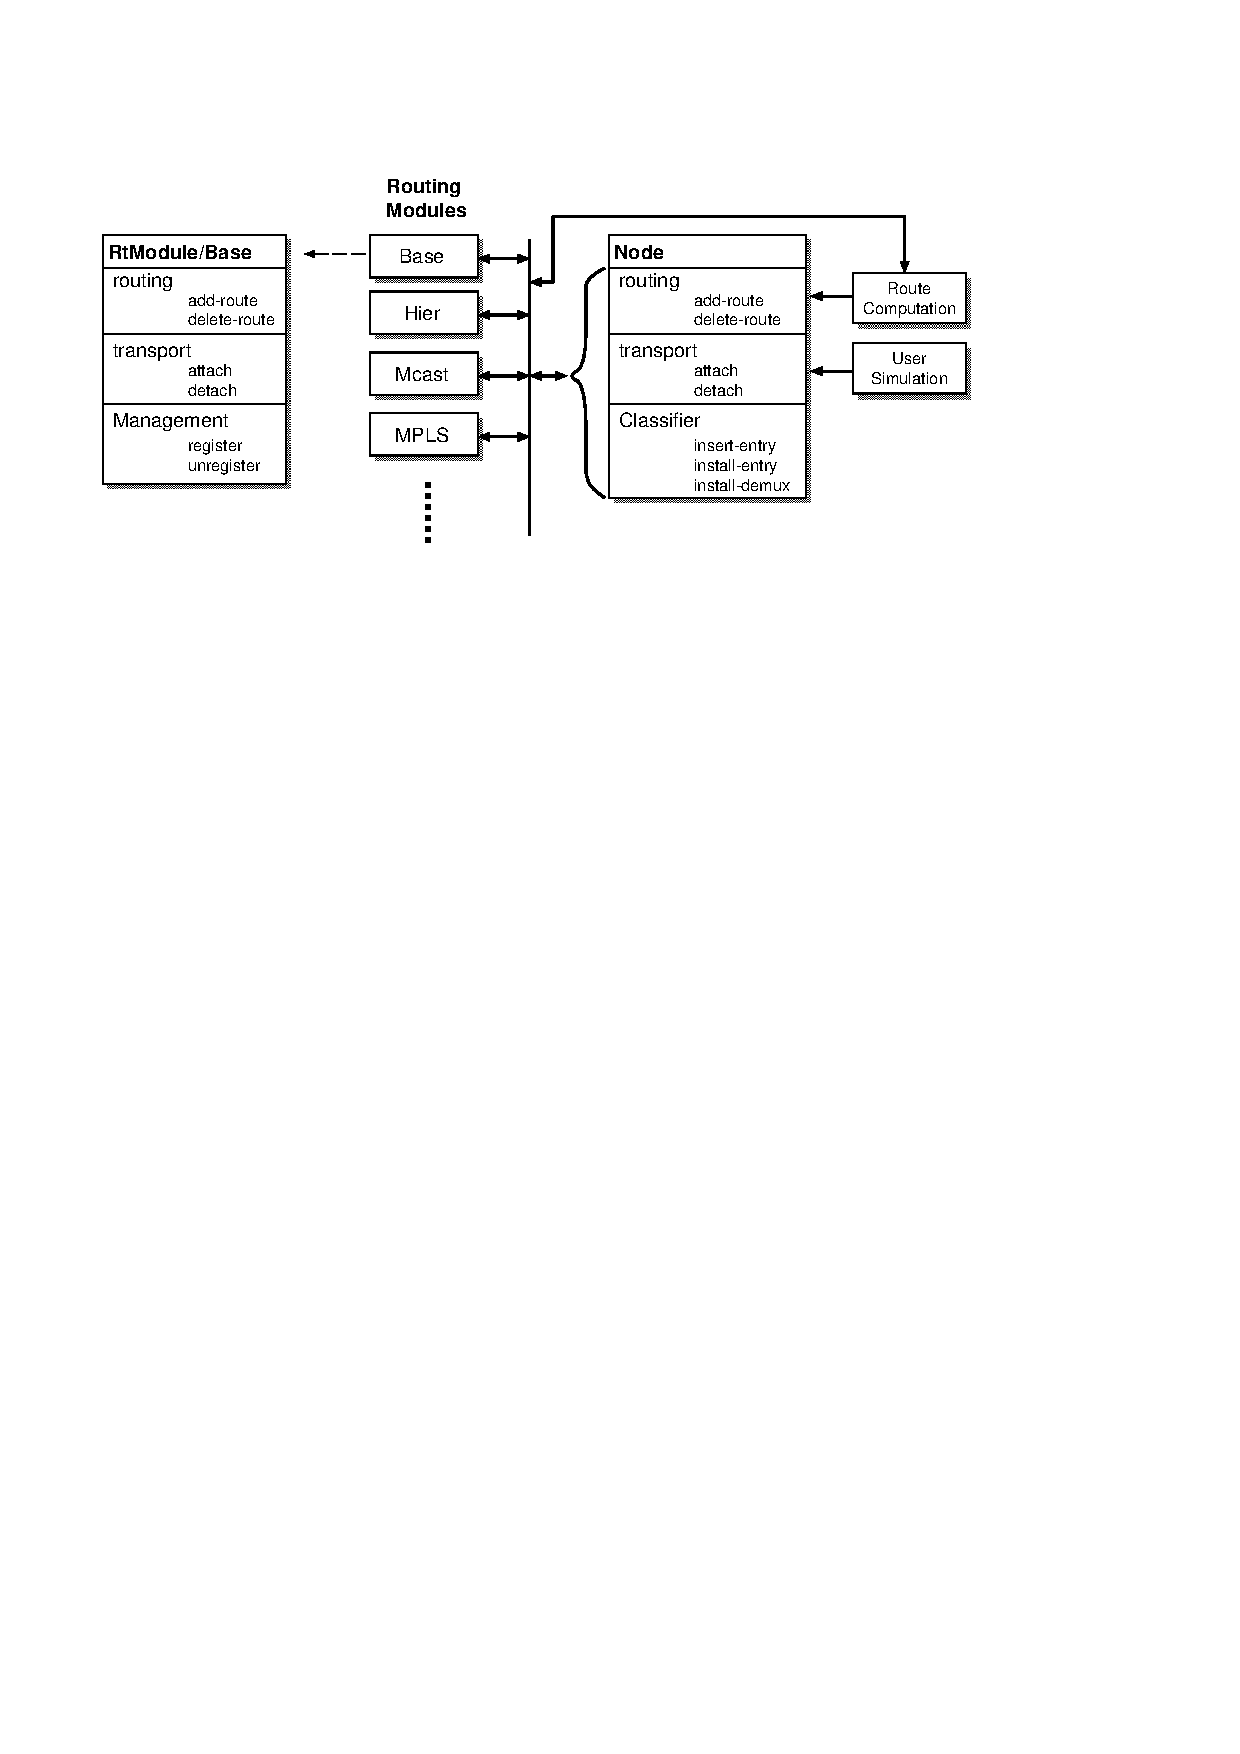
\includegraphics{rtmodule}
    \caption{Interaction among node, routing module, and routing. The
      dashed line shows the details of one routing module.}
    \label{fig:node:rtmodule}
  \end{center}
\end{figure}

When a new routing protocol implementation includes more than one
function blocks, especially when it contains its own classifier, it is
desirable to have another object, which we call 
a {\em routing module}, that manages all these function 
blocks and to interface with node to organize its classifiers.
Figure~\ref{fig:node:rtmodule} shows functional relation among these
objects.
Notice that routing modules may have direct relationship with route
computation blocks, i.e., route logic and/or routing agents.
However, route computation MAY not install their routes directly
through a routing module, because there may exists other modules that
are interested in learning about the new routes.
This is not a requirement, however, because it is possible that some
route computation is specific to one particular routing module, for
instance, label installation in the MPLS module. 

A routing module contains three major functionalities:
\begin{enumerate}
\item %Management
  A routing module initializes its connection to a node through
  \proc[]{register}, and tears the connection down via
  \proc[]{unregister}.
  Usually, in \proc[]{register} a routing module (1) tells the node
  whether it
  interests in knowing route updates and transport agent attachments,
  and (2) creates its classifiers and install them in the node
  (details described in the next subsection).
  In \proc[]{unregister} a routing module does the exact opposite: it
  deletes its classifiers and removes its hooks on routing update in
  the node.
\item %Route handler
  If a routing module is interested in knowing routing updates, the
  node will inform the module via \\
  \proc[dst, target]{RtModule::add-route} and
  \proc[dst, nullagent]{RtModule::delete-route}.
\item %Transport agent handler
  If a routing module is interested in learning about transport agent
  attachment and detachment in a node, the node will inform the module
  via \\ 
  \proc[agent, port]{RtModule::attach} and
  \proc[agent, nullagent]{RtModule::detach}.
\end{enumerate}

There are two steps to write your own routing module:
\begin{enumerate}
\item You need to declare the C++ part of your routing
  module (see \nsf{rtmodule.\{cc,h\}}). For many modules this only
  means to declare a virtual method \code{name()} which returns a
  string descriptor of the module. However, you are free to implement
  as much functionality as you like in C++; if necessary you may
  later move functionality from OTcl into C++ for better performance. 
\item You need to look at the above interfaces implemented in the base
  routing module (see \nsf{tcl/lib/ns-rtmodule.tcl}) and decide which
  one you'll inherit, which one you'll override, and put them in OTcl
  interfaces of your own module. 
\end{enumerate}
There are several derived routing module examples in
\nsf{tcl/lib/ns-rtmodule.tcl}, which may serve as templates for your
modules.

Currently, there are six routing modules implemented in \ns:
\begin{table}[htbp]
  \begin{center}
    \begin{tabular}[htbp]{|c|p{5in}|}
      \hline
      Module Name & Functionality \\ 
      \hline \hline
      RtModule/Base & Interface to unicast routing protocols. Provide
        basic functionality to add/delete route and attach/detach
        agents. \\ \hline
      RtModule/Mcast & Interface to multicast routing protocols. Its
        only purpose is establishes multicast classifiers. All other
        multicast functionalities are implemented as instprocs of
        Node. This should be converted in the future. \\ \hline
      RtModule/Hier & Hierarchical routing. It's a wrapper for
        managing hierarchical classifiers and route installation. Can
        be combined with other routing protocols, e.g., ad hoc
        routing. \\ \hline
      RtModule/Manual & Manual routing. \\ \hline
      RtModule/VC & Uses virtual classifier instead of vanilla
        classifier. \\ \hline
      RtModule/MPLS & Implements MPLS functionality. This is the only
        existing module that is completely self-contained and does not
        pollute the Node namespace. \\
      \hline
    \end{tabular}
    \caption{Available routing modules}
    \label{tab:node:rtmodule}
  \end{center}
\end{table}

\subsection{Node Interface}

To connect to the above interfaces of routing module, a node provides
a similar set of interfaces:
\begin{itemize}
\item %Management
  In order to know which module to register during creation, the Node
  class keeps a list of modules as a class variable. 
  The default value of this list contains only the base routing
  module.
  The Node class provides the following two {\em procs} to manipulate
  this module list:
  \begin{alist}
    \proc[name]{Node::enable-module} & If module
    \code{RtModule/[name]} exists, this proc puts [name] into the
    module list. \\ 
    \proc[name]{Node::disable-module} & If
    [name] is in the module 
    list, remove it from the list. 
  \end{alist}
  When a node is created, it goes through the module list of the Node
  class, creates all modules included in the list, and register these
  modules at the node.

  After a node is created, one may use the following instprocs to list
  modules registered at the node, or to get a handle of a module with
  a particular name:
  \begin{alist}
    \proc[]{Node::list-modules} & Return a list of the handles (shadow
    objects) of all registered modules. \\
    \proc[name]{Node::get-module} & Return a
    handle of the 
    registered module whose name matches the given one. Notice that
    any routing module can only have a single instance registered at
    any node.
  \end{alist}
\item %route and port
  To allow routing modules register their interests of routing
  updates, a node object provide the following instprocs:
  \begin{alist}
    \proc[module]{Node::route-notify} & Add \code{module} into route
    update notification list. \\
    \proc[module]{Node::unreg-route-notify} & Remove \code{module}
    from route update notification list. \\
  \end{alist}
  Similarly, the following instprocs provide hooks on the attachment
  of transport agents:
  \begin{alist}
    \proc[module]{Node::port-notify} & Add \code{module} into agent
    attachment notification list. \\
    \proc[module]{Node::unreg-port-notify} & Remove \code{module} from
    agent attachment notification list. \\
  \end{alist}
  Notice that in all of these instprocs, parameter \code{module}
  should be a module handle instead of a module name. 
\item %classifier
  Node provides the following instprocs to manipulate its address and
  port classifiers:
  \begin{itemize}
  \item \proc[module, clsfr, hook]{Node::insert-entry} inserts
    classifier \code{clsfr} into the entry point of the node. It also
    associates the new classifier with \code{module} so that if this
    classifier is removed later, \code{module} will be unregistered.
    If \code{hook} is specified as a number, the existing classifier
    will be inserted into slot \code{hook} of the new classifier. 
    In this way, one may establish a ``chain'' of classifiers; see
    Figure~\ref{fig:node:multicast} for an example.
    {\bf NOTE}: \code{clsfr} needs NOT to be a classifier. In some
    cases one may want to put an agent, or any class derived from
    Connector, at the entry point of a node. In such cases, one simply
    supplies \code{target} to parameter \code{hook}.
  \item \proc[module, clsfr, hook]{Node::install-entry} differs from
    \code{Node::insert-entry} in that it deletes the existing
    classifier at the node entry point, unregisters any associated
    routing module, and installs the new classifier at that point. 
    If \code{hook} is given, and the old classifier is connected into
    a classifier chain, it will connect the chain into slot
    \code{hook} of the new classifier. 
    As above, if \code{hook} equals to \code{target}, \code{clsfr}
    will be treated as an object derived from Connector instead of a
    classifier. 
  \item \proc[demux, port]{Node::install-demux} places the given
    classifier \code{demux} as the default demultiplexer. If
    \code{port} is given, it plugs the existing demultiplexer into
    slot \code{port} of the new one. Notice that in either case it does
    not delete the existing demultiplexer.
  \end{itemize}
\end{itemize}

\section{Commands at a glance}
\label{sec:nodescommand}
\begin{flushleft}

Following is a list of common node commands used in simulation scripts:

\code{$ns_ node [<hier_addr>]}\\ %$
Command to create and return a node instance. If <hier\_addr> is given,
assign the node address to be <hier\_addr>. Note that the latter MUST
only be used when hierarchical addressing is enabled via either
\proc[]{set-address-format hierarchical} or 
\proc[]{node-config -addressType hierarchical}. 

\code{$ns_ node-config -<config-parameter> <optional-val>}\\%$
This command is used to configure nodes. The different config-parameters
are addressingType, different type of the network stack components,
whether tracing will be turned on or not, mobileIP flag is truned or not,
energy model is being used or not etc. An option -reset maybe used to set
the node configuration to its default state. The default setting of 
node-config, i.e if no values are specified, creates a simple node (base
class Node) with flat addressing/routing. For the syntax details see
Section~\ref{sec:node:nodeconfig}.

\code{$node id}\\%$
Returns the id number of the node.

\code{$node node-addr}\\%$
Returns the address of the node. In case of flat addressing, the node address
is same as its node-id. In case of hierarchical addressing, the node address
in the form of a string (viz. "1.4.3") is returned.

\code{$node reset} \\%$
Resets all agent attached to this node.

\code{$node agent <port_num>} \\%$
Returns the handle of the agent at the specified port. If no agent is found
at the given port, a null string is returned.

\code{$node entry}\\%$
Returns the entry point for the node. This is first object that
handles packet receiving at this node.

\code{$node attach <agent> <optional:port_num>}\\%$
Attaches the <agent> to this node. Incase no specific port number is passed,
the node allocates a port number and binds the agent to this port. Thus once
the agent is attached, it receives packets destined for this host
(node) and port. 

\code{$node detach <agent> <null_agent>}\\%$
This is the dual of "attach" described above. It detaches the agent
from this node 
and installs a null-agent to the port this agent was attached. This is
done to handle transit packets that may be destined to the detached
agent. These on-the-fly packets are then sinked  at the null-agent.

\code{$node neighbors}\\%$
This returns the list of neighbors for the node.

\code{$node add-neighbor <neighbor_node>}\\%$
This is a command to add \code{<neighbor_node>} to the list of neighbors 
maintained by the node.

\rule{\linewidth}{0.3mm}
Following is a list of internal node methods:

\code{$node add-route <destination_id> <target>}\\%$
This is used in unicast routing to populate the classifier. The target is a
Tcl object, which may be the entry of \code{dmux_} (port demultiplexer in
the node) incase the \code{<destination_id>} is same as this node-id.
Otherwise it is usually the head of the link for that destination. It
could also be the entry for other classifiers.

\code{$node alloc-port <null_agent>}\\%$
This returns the next available port number.

\code{$node incr-rtgtable-size}\\%$
The instance variable \code{rtsize_} is used to keep track of size of
routing-table in each node. This command is used to increase the
routing-table size every time an routing-entry is added to the
classifiers.

There are other node commands that supports hierarchical
routing, detailed dynamic routing, equal cost multipath
routing, manual routing, and energy model for mobile nodes. These
and other methods described earlier can be found in 
\nsf{tcl/lib/ns-node.tcl} and \nsf{tcl/lib/ns-mobilenode.tcl}.

\end{flushleft}
\endinput
% LocalWords:  ns tcl lib rtmodule addr cc mcast mpath replicator unicast pt ht
% LocalWords:  multicast mcastNode TclObject dmux installNext strcmp argv int
% LocalWords:  atoi NsObject NsObject argc recv instproc OTcl AddressClassifier
% LocalWords:  const IPHeader IPHeader dst nsaddr Otcl MCastClassifierClass src
% LocalWords:  TclClass MCastClassifier findslot struct hashnode pkt XXX evalf
% LocalWords:  MultiPath multipath MultiPathForwarder cl ip flowid ip NodeShift
% LocalWords:  NodeMask AddrParams SrcDest Dest SrcDestFid hashcl nbuck IDs del
% LocalWords:  flor bj LANs iph maxslot Hier onsists tb MPLS RtModule nullagent
% LocalWords:  config config val num alloc incr rtgtable
